\chapter{Inflationary Cosmology}
\label{chap:cos}

\section{Introduction}
\label{sec:cos:intro}

\section{Conventions}
\label{sec:cos:conventions}


\begin{enumerate}
  \item I work using a metric with a positive signature $(+,-,-,-)$.
  \item Fourier transforms are written with an overloaded notation, and defined so that Fourier synthesis carries the factors of $2\pi$:
    \begin{equation}
      f(\vk) = \int_{-\infty}^{\infty} d^3\vx\: e^{-i \vk\cdot\vx} f(\vx) \qquad f(\vx) = \int_{-\infty}^{\infty} \frac{d^3\vk}{{(2\pi)}^3}\: e^{i \vx\cdot\vk} f(\vk).
      \label{eqn:cos:fourier_transform}
    \end{equation}
  \item I work in natural units so that 
    \begin{equation}
      c = \hbar = G = k_B = 1,
      \label{eqn:cos:natural_units}
    \end{equation}
    but retain the reduced Planck mass for clarity:
    \begin{equation}
      \m = \frac{1}{8\pi G}.
      \label{eqn:cos:reduced_planck_mass}
    \end{equation}
    
\end{enumerate}


\section{Einstein's gravity}
\label{sec:cos:einsteins_gravity}

Einstein's gravity can be effectively summarised using the Einstein-Hilbert action formalism. An action $S$ is written as a general relativistic integral over a Lagrangian density $\mathcal{L}$:\footnote{This should not be confused with a likelihood, also denoted with $\lik$.}
\begin{equation}
  S = \int d^4 x \sqrt{|g|} \mathcal{L}.
  \label{eqn:cos:generic_lagrangian}
\end{equation}
note that the factor of $\sqrt{|g|}$, $g=\det(g_{\mu\nu})$ ensures a relativistic volume element for integration.
We typically decompose the Lagrangian $\mathcal{L}$ into a gravitational and matter part:
\begin{align}
  \mathcal{L} &= \mathcal{L}_G + \mathcal{L}_M
  \label{eqn:cos:decomp}\\
  \mathcal{L}_G &= \frac{1}{2} \m^2 R
  \label{eqn:cos:L_grav}
\end{align}
where $g=\det(g_{\mu\nu})$ is the determinant of the metric, $R$ is the Ricci scalar~\eqref{eqn:dg:ricci_scalar}, and $\mathcal{L}_M$ is the portion of the Lagrangian pertaining to the material contents of the spacetime. Requiring that the action~\eqref{eqn:cos:generic_lagrangian} is extremal ($\delta S = 0$) yields Einstein's equations:
\begin{equation}
 \m^2 G_{\mu\nu} = T_{\mu\nu},
  \label{eqn:cos:einsteins_equations}
\end{equation}
where
\begin{equation}
  T_{\mu\nu} = \frac{-2}{\sqrt{\abs{g}}}\frac{\delta}{\delta g^{\mu\nu}}\left( \sqrt{\abs{g} \mathcal{L}_M} \right)
  \label{eqn:cos:SET_fundamantal}
\end{equation}
is the stress energy tensor, and
\begin{equation}
  G_{\mu\nu} = R_{\mu\nu} - \frac{1}{2}g_{\mu\nu} R,
  \label{eqn:cos:SET_fundamantal}
\end{equation}
is the Einstein tensor.

\section{Friedman-Robertson-Walker spacetime}

Cosmological principle:
\begin{quote}
  At any particular time, the universe looks the same in all directions from any position in space.
\end{quote}

On the largest scales, the universe is observed to be {\em homogeneous\/} and {\em isotropic}.
\begin{equation}
  ds^2 = dt^2 - a{(t)}^2\left( d\chi^2 + S^2{(\chi)} d\Omega \right)
  \label{eqn:cos:FRW_metric}
\end{equation}

\section{The $\Lambda$CDM concordance cosmology}

\begin{figure}
\centerline{%
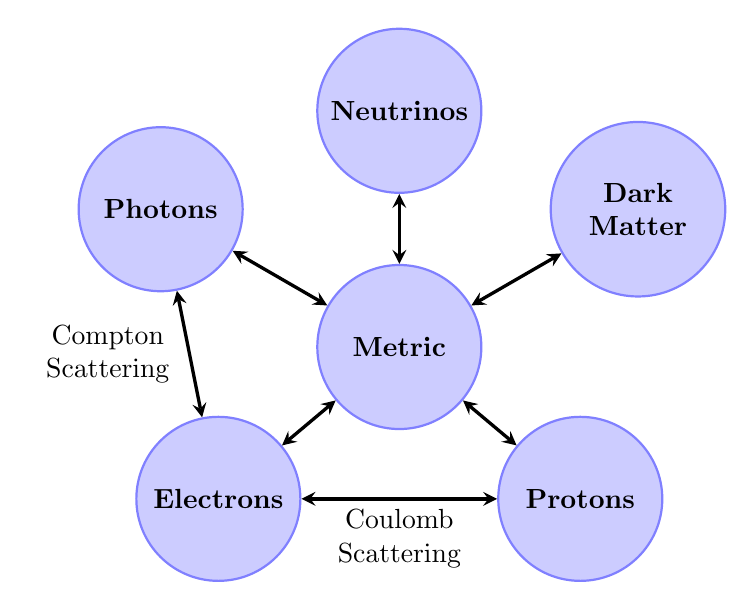
\begin{tikzpicture}[%
    writing/.style={%
      text width=18mm,  % default text width
      align=center      % align in center
    },
    component/.style={%
      circle,           % circular node
      fill=blue!20,     % fill it in blue
      draw=blue!50,     % outside edge in blue
      thick,            %              and thick
      writing,          % writing style above
      font=\bfseries    % bold writing
    },
    connection/.style={%
      <->,             % Double headed
      very thick,      % very thick arrows
      >=stealth        % pretty arrow head
    }
]

    % nodes
    \node at (0,0)     [component] (metric)      {Metric};

    \node at (90 :3)   [component] (neutrinos)   {Neutrinos};
    \node at (150:3.5) [component] (photons)     {Photons};
    \node at (220:3)   [component] (electrons)   {Electrons};    
    \node at (320:3)   [component] (protons)     {Protons};      
    \node at (30 :3.5) [component] (dark matter) {Dark Matter};


    % connections
    \draw[connection] (metric) -- (neutrinos);
    \draw[connection] (metric) -- (photons);
    \draw[connection] (metric) -- (electrons);
    \draw[connection] (metric) -- (protons);
    \draw[connection] (metric) -- (dark matter);

    % interconnections with text
    \draw[connection] 
    (electrons) to 
    node[below,writing] {Coulomb Scattering} 
    (protons);

    \draw[connection] 
    (electrons) to 
    node[left,writing] {Compton Scattering} 
    (photons);

\end{tikzpicture}

}
\caption{Composition of the universe, along with the interaction of the components.\label{fig:cos:composition}}
\end{figure}


\section{The horizon problem}

\section{Inflation}


\clearpage{}

\section{Scalar field inflation models}
\label{sec:Scalar_field_inflation_models}
%
A universe comprised of multiple components  with densities
$\{\rho_i\}$ and pressures $\{P_i\}$ has the evolution equations
%
\begin{align}
  \dot{H}+H^2 &= 
  -\frac{1}{6\m^2}\sum\limits_i\left( \rho_i + 3P_i\right), 
  \label{eqn:Raychaudhuri_rho}
  \\
  H^2 &= 
  \frac{1}{3\m^2}\sum\limits_i \rho_i, 
  \\
  \dot{\rho}_i 
  &= -3(\rho_i + P_i)H,  
  \label{eqn:conservation}
\end{align}
%
where $H=\dot{a}/a$ is the Hubble parameter, $a$ is the normalized scale factor and a dot denotes differentiation with respect to cosmic time, $\dot{f}\equiv df/dt$. The first equation is the {\em Raychaudhuri\/} equation, and is derived from the trace of the Einstein equations. The second is the {\em Friedmann\/} equation and represents the conservation of energy. The third is the {\em continuity\/} equation for the fluid $\rho_i$. It should be noted that these equations are not independent, and that the Raychaudhuri equation may be straightforwardly derived from the Friedmann and continuity equations.  For convenience, we use Planck units ($G=c=\hbar=1$) throughout, but for clarity retain the reduced Planck mass: 
%
\[\m = \sqrt{\frac{\hbar c}{8\pi G}} = {(8\pi)}^{-1/2}.\]  
%


The simplest way to create a homogeneous and isotropic cosmological background model which undergoes an inflationary phase is by assuming that one of the fields is a real, time-dependent and homogeneous scalar field $\phi(t)$. The energy density and pressure of such a field is given by 
%
\begin{equation}
  \rhoph = \tfrac{1}{2}\dot{\phi}^2+V(\phi),
  \qquad
  \Pph = \tfrac{1}{2}\dot{\phi}^2-V(\phi).
  \label{eqn:rhopdef}
\end{equation}
%
In addition to the scalar field, we shall allow the possibility of including a collection of additional noninteracting fluids with densities $\{\rho_i\}$ and pressures $\{P_i\}$ defined by their equation-of-state parameters:
%
\begin{equation}
  w_i =\frac{P_i}{\rho_i},
  \label{eqn:equation_of_state}
\end{equation}
%
where ${w_i}$ are a set of constants determining the type of each fluid. Some commonly assumed cosmological fluids are listed in Table~\ref{tab:type_of_fluid} along with their $w$-values. Note that we are accommodating the possibility of spatially curved universes implicitly by including the case $w_i=-1/3$. We shall term all of these {\em auxiliary fluids}.
%
\begin{table}
  \centerline{%
    \begin{tabular}{lc}
      \toprule
      Type of fluid & $w$ \\
      \midrule
      Scalar field during KD & $ \phantom{-}1\phantom{/3} $ \\
      Radiation & $ \phantom{-}1/3 $ \\
      Matter & $ \phantom{-}0\phantom{/3} $ \\
      Spatial curvature & $ -1/3$ \\
      Missing matter & $ -2/3$ \\
      Dark energy (cosmological constant) & $ -1\phantom{/3} $ \\
      \bottomrule
    \end{tabular}
  }
  \caption{Commonly assumed cosmological fluids and their
    equation-of-state parameters $w$, defined by equation equation (\protect\ref{eqn:equation_of_state}).  For more information on ``missing matter'', see \protect\citet{vazquez_2012}\label{tab:type_of_fluid}.
  }
\end{table}
%

Using the notation in~\eqref{eqn:equation_of_state} and defining the present-day densities $\{\rho_{i,0}\}$, the evolution equations~\eqref{eqn:Raychaudhuri_rho,eqn:conservation} take the form 
%
\begin{align}
  \dot{H}+H^2 &= 
  -\frac{1}{3\m^2}\left[\dot{\phi}^2 - V(\phi) +
  \sum_i\tfrac{1}{2}(1+3w_i)\rho_i\right] ,
  \label{eqn:Raychaudhuri_mod}
  \\
  H^2 &= 
  \frac{1}{3\m^2}\left[\tfrac{1}{2}\dot{\phi}^2 + V(\phi) +
  \sum_i\rho_i\right],
  \label{eqn:Friedmann_mod} 
  \\
  \rho_i &= 
  \rho_{i,0} \,a^{-3(1+w_i)},
  \label{eqn:rho_a} 
  \\ 
  0&= 
  \ddot{\phi} +3\dot{\phi}H + V^\prime(\phi).
  \label{eqn:Klein_Gordon_mod}
\end{align}
%                                                          

Inflation is defined as $\ddot{a}>0$, or equivalently as $\dot{H}+H^2>0$. In the case when only an inflaton is present, this condition can be recast in terms of the scalar field using the Raychaudhuri equation~\eqref{eqn:Raychaudhuri_mod} as
%
\begin{equation}
  \dot{\phi}^2<V(\phi).
  \label{eqn:Onset_inflation}
\end{equation}
%
The slow-roll inflation regime satisfies
%
\begin{equation}
  \dot{\phi}^2\ll V(\phi).
  \label{eqn:Slow-roll}
\end{equation}
%
The amount of inflation is measured by the number of $e$-folds $N\propto \log a$, which is related to the Hubble parameter $H$ by
%
\begin{equation}
  \dot{N}=H.\label{eqn:e-folds}
\end{equation}
%

For a generic potential $V(\phi)$, there is no analytic solution for the dynamics of a scalar field inflation model, even if no other fluids are present. Hence, even in this simple case, the evolution equations~\eqref{eqn:Raychaudhuri_mod} and~\eqref{eqn:Klein_Gordon_mod} have to be integrated numerically using suitable ``initial'' conditions at some time $t=\ti$. In principle, $t=\ti$ may be {\em any\/} cosmic time, although numerical stability of the solution usually requires that the conditions be specified prior to the onset of inflation.  Once any two of $\phii \equiv \phi(\ti)$, $\dot{\phii} \equiv \dot{\phi}(\ti)$ and $\Hi \equiv H(\ti)$ have been specified, the Friedmann equation~\eqref{eqn:Friedmann_mod} yields the third. The quantities $\Hi$, $\phii$ and $\dot{\phii}$ then provide the necessary initial conditions for the integration of the coupled dynamical equations~\eqref{eqn:Raychaudhuri_mod} and~\eqref{eqn:Klein_Gordon_mod} for $\phi(t)$ and $H(t)$.


\section{Background}
\label{sec:background}

\clearpage{}

We denote a general action via
\begin{equation}
  S_I = \int d^4x\sqrt{|g|}\mathcal{L}_I,
  \label{eqn:general_action}
\end{equation}
where $\mathcal{L}_I$ is the {\em Lagrangian density}. We work in natural units $\hbar=c=1$ and set the reduced Planck mass $m_\mathrm{p} = {(8\pi G)}^{-1/2} = 1$. Dots denote differentiation with respect to cosmic time $\dot{f}\equiv \frac{d}{dt}f$, and primes denote differentiation with respect to conformal time $\prm{f}\equiv\frac{d}{d\eta}f$.

We begin by briefly summarising the classical theory of cosmological perturbations for a general scalar field, before discussing the quantisation of such a theory


\subsection{The classical action}
\label{sec:inflation}
Consider~\cite{Baumann+2009} a canonical scalar field $\phi$ minimally coupled to gravity $S= S_G + S_\phi$ with:
\begin{equation}
  \mathcal{L}_G = \frac{1}{2}R, 
  \qquad
  \mathcal{L}_\phi = \frac{1}{2}g^{\mu\nu}\nabla_\mu\phi\nabla_\nu\phi - V(\phi),
  \label{eqn:action}
\end{equation}
Extremising this action with respect to the fields $\phi$ and $g_{\mu\nu}$ recovers the Klein-Gordan and Einstein equations respectively:
\begin{align}
  \left( g^{\mu\nu}\nabla_\mu\nabla_\nu + \frac{dV}{d\phi} \right) \phi &= 0,
  \label{eqn:klein_gordon}\\
  G_{\mu\nu}\equiv R_{\mu\nu}-\frac{1}{2}g_{\mu\nu}R&= T_{\mu\nu},
  \label{eqn:einstein}
\end{align}
where the stress-energy tensor is:
\begin{equation}
  T_{\mu\nu} = \nabla_\mu\phi \nabla_\nu\phi - \frac{1}{2}g_{\mu\nu} \nabla_\alpha\phi \nabla^\alpha\phi +g_{\mu\nu} V(\phi).
  \label{eqn:SET}
\end{equation}

In cosmology, we assume that at zeroth order both the metric $g_{\mu\nu}$ and scalar field $\phi$ are homogeneous and isotropic. Applying these assumptions to equations~\eqref{eqn:klein_gordon}~\&~\eqref{eqn:einstein}, we find:
\begin{align}
  \dot{H}+H^2 &= -\frac{1}{3}\left( \dot{\phi}^2 - V(\phi) \right),
  \label{eqn:Raychaudhuri}\\
  0&=\ddot{\phi} + 3H\dot{\phi} + \frac{dV}{d\phi},
\end{align}
where the Hubble parameter $H = \dot{a}/a$.
